%\chapter{sciencetech}

%%%%%%%%%%%%%%%%%%%%%%%%%%%%%%%%%%%%%%%%%%%%%%
\section{Overview}
\fixme{Anne added this section 7/28; there needs to be a general intro. I've borrowed this text from CDR detector vol, sec 9.3.1) }

As an \textit{engineering} prototype, ProtoDUNE-SP is
intended to validate the construction of the components planned for the
first DUNE \ktadj{10} detector module at scale and thereby mitigate
risks associated with extrapolating small-scale versions of the
single-phase LArTPC technology to a full 10-kt detector module.  It is
intended to benchmark the operation of full-scale detector
elements and perform measurements in a well characterized
charged-particle beam --- an essential step.

The prototype will incorporate components with the same
dimensions and features as those for the first 10-kt DUNE far detector
module.

Besides validating the performance of the detector components,
planning and constructing the CERN prototype will establish and
commission production sites and test the installation procedure.
Further, before the beam test, many basic detector-performance
parameters can be established with cosmic-ray muons.  These data will
aid in identification of potentially problematic components, leading
to future improvements and optimizations of the detector design.  Once
it is exposed to a test beam of charged particles of different types
and energies it will collect data that can be combined with results
from LArIAT and the short-baseline program at Fermilab.  Together
these measurements will be used to validate MC simulations, and they
will serve as data input to DUNE sensitivity studies and allow
validation and tuning of tools for event reconstruction and particle
identification.

%%%%%%%%%%%%%%%%%%%%%%%%%%%%%%%%%%%%%%%%%%%%%%
\section{Charged particle beam studies}
\fixme{Science description?}

One of the crucial goals of the ProtoDUNE-SP experiment is to measure and study the response of the detector to charged
particles of different types and energies. Results from these measurements serve to
assess systematic detector uncertainties and validate Monte Carlo (MC) simulations. They also enable
validation and tuning of event reconstruction algorithms and particle identification tools.
\fixme{If we keep new overview, the above is already said}

The DUNE experiment will run in both neutrino and antineutrino 
configurations. These beams will be composed mainly of muon neutrinos (antineutrinos) as well as electron neutrinos (antineutrinos). In Fig.~\ref{fig:particle_momenta} the momentum distributions particles created in neutrino interactions from simulated beam fluxes, including oscillation effects, are shown. The particle rates are normalized  to the number of neutrino interactions in the DUNE far detector and the neutrino beam flux. \fixme{Need a sentence that connects this DUNE info with ProtoDUNE charged particle beam test better.}

\begin{cdrfigure}[Placeholder: Momentum distributions]{particle_momenta}{Placeholder: Left: Momentum distributions of particles produced by the neutrinos from the neutrino beam in DUNE. Right: the predicted rate of particles as a function of their momentum for the charged particle beamline (at CERN???).} 
  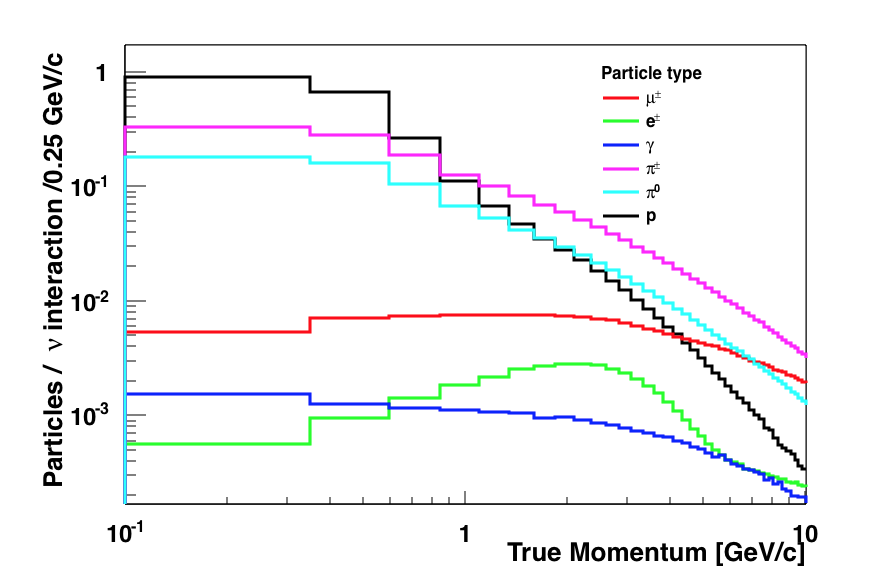
\includegraphics[width=0.8\textwidth]{True_Momenta_per_Particle_9_2_1_0_logy_logx}
\end{cdrfigure}

The main ProtoDUNE-SP studies that will be performed using charged particles from the beam and particles created by cosmic muons are
\fixme{Each of the point below will be described in details in the next draft.}
\begin{description}
\item [Characterization of hadronic showers (high $p$) and topologies of hadronic interactions (low $p$).]
% was too long \item [Characterization of hadronic showers (high momenta) and  topologies of the hadronic interactions (low momenta).]

Accurate measurement of neutrino energy will require reconstruction of both electromagnetic and hadronic showers. Reconstruction of hadron energy 
in these energy ranges will require knowledge of the fate (interact, decay, or stop) of the
initiating hadron ($\pi^{+/-}$, $p$, or $K^{+/-}$).
For the case of  interacting hadrons, the composition of secondaries
will need to be determined to characterize the response. 
These will include neutrals and particles that 
deposit energy electromagnetically ($\pi^o$, $\gamma$), as well as
secondary hadrons.
The test beam with known incoming particle type and momentum will be used
to characterize interacting hadrons in this energy range.


Fig.~\ref{fig:hadronshwr} shows the fraction of true energy deposited by interacting protons with 1~GeV/c (left) and
3~GeV/c (right) incident momenta simulated using FLUKA particle transport code~\cite{fluka05}. 
Interacting protons (65\% of the 1~GeV/c sample) are selected.
For this study, visible energy is summed using hit information with corrections applied for the lifetime of 
the drift electrons (No attempt is made to correct for recombination effects or electromagnetic shower fractions). 
The resulting energy deposition in the two cases cannot be 
accurately characterized by an average shower calibration factor. MC simulations of 
outgoing particles, especially at low energies, must be checked and bench-marked against calibration data to avoid
large uncertainties from shower modeling. 

\begin{cdrfigure}[Fraction of true energy deposited by interacting protons of 1~GeV/c and
3~GeV/c]{hadronshwr}{Fraction of true energy deposited by interacting protons of 1~GeV/c (left) and
3~GeV/c (right) momenta simulated using FLUKA~\cite{fluka05}.}
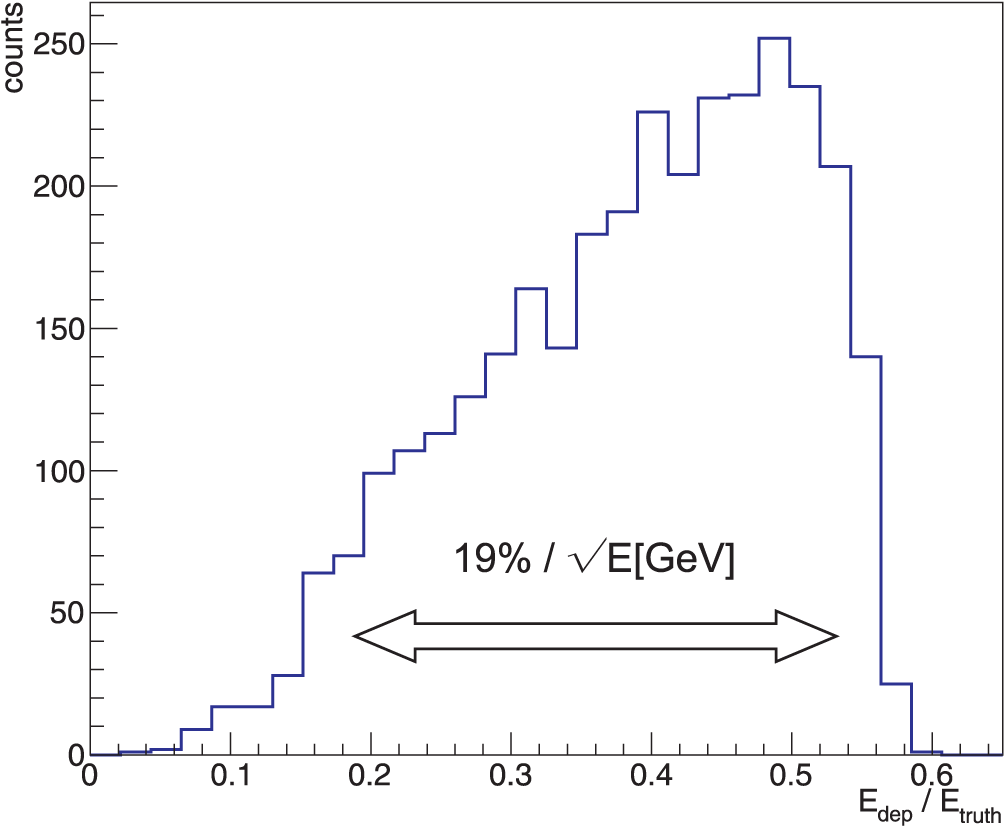
\includegraphics[width=0.49\textwidth,height=5.0cm]{pr1GeV_v2a}
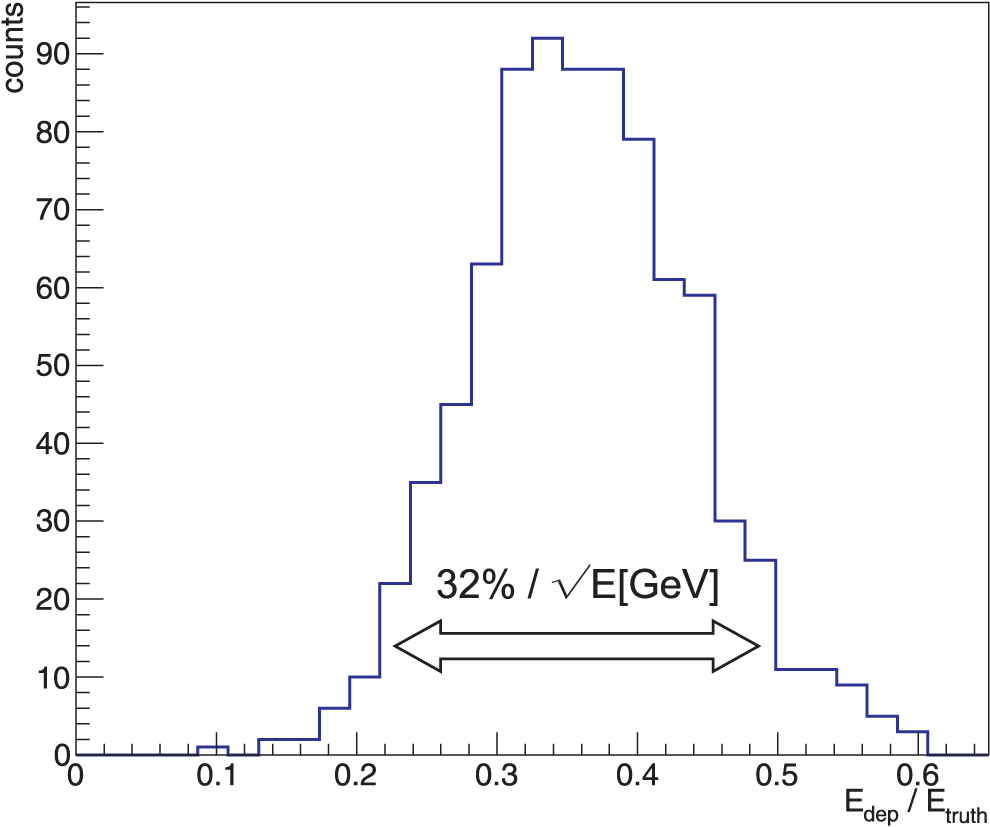
\includegraphics[width=0.49\textwidth,height=5.0cm]{pr3GeV_v2a}
\end{cdrfigure}


Pion showers at low energies will also be important both for determining the interacted neutrino energy and for modeling neutral current backgrounds resulting from $\pi^o$ content in showers. Significant
 differences in energy deposited in interactions initiated
by $\pi^+$ versus $\pi^-$  are present up to momenta on the order of 1~GeV/c due to different
final-state particles and interaction cross sections. This is illustrated in 
Fig.~\ref{fig:pionshwr}, which shows the differences in mean energy deposited (left) and width (right) 
for interacting pions with momenta ranging from 0.2~GeV/c up to 5~GeV/c.
Resulting shower calibrations and reconstruction will differ; therefore each charge must be 
studied separately.

\begin{cdrfigure}[Differences in mean energy deposited and width of visible energy, 
 $\pi^+$ versus $\pi^-$]{pionshwr}{Differences in mean energy deposited (left) and width of visible energy (right) 
for interacting $\pi^+$ versus $\pi^-$ ranging from 0.2~GeV/c up to 5~GeV/c. }
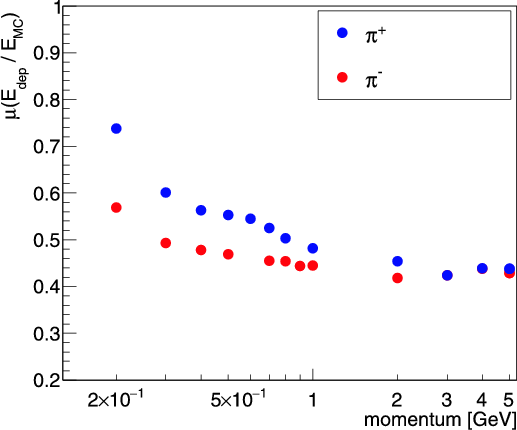
\includegraphics[width=0.49\textwidth,height=6.0cm]{pipimean_ticks1}
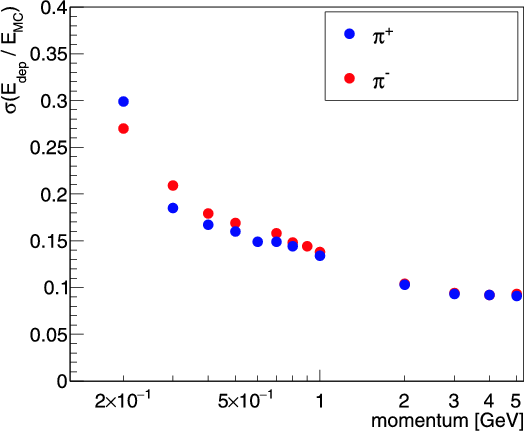
\includegraphics[width=0.49\textwidth,height=6.0cm]{pipisigma_ticks1}
\end{cdrfigure}


\item [Characterization of electromagnetic showers]
\fixme{some text?}
\item [Study of $e/\gamma$ separation capabilities]

The search for a CP violation phase using $\nu_e$ appearance 
in a $\nu_\mu$ beam requires good electron/photon separation.
Backgrounds originating from photons produced primarily from 
final state $\pi^0$'s must be identified and removed from the signal
electron sample. 

High-energy photons can undergo two processes: pair production and Compton scattering. 
The dominant process for photons with energies of several hundred MeV or more is 
e$^+$ e$^-$ pair production.
%energies. 
%For pair production the 
For this process e/$\gamma$ discrimination
 can be achieved using the beginning of the electromagnetic shower, where 
a single MIP is characteristic of electron energy deposition, while two MIPs would be consistent 
with Compton scattering. %a photon hypothesis.
In the latter case %where the photon Compton-scatters, the two particles 
the two MIPs cannot easily be distinguished
from the energy deposition pattern.

\begin{cdrfigure}[Photon background rejection versus electron identification efficiency for various energies]{egam}{Photon background rejection versus electron identification efficiency for various energies, calculated for and normalized to samples which pass the reconstruction. 
The simulation was performed in APA design configuration (4.67-mm wire pitch, induction wires at $\pm$35.7$^{\circ}$ w.r.t. collection wires).}
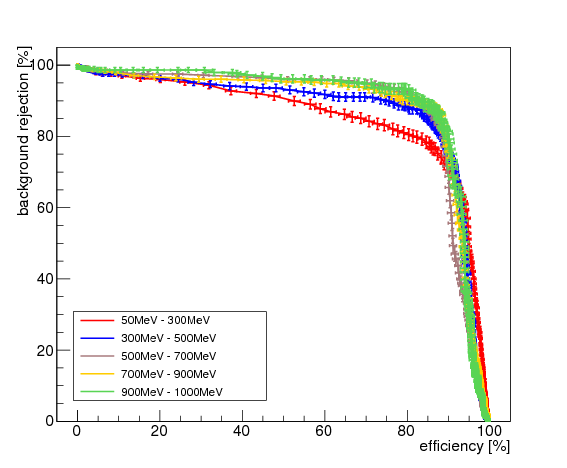
\includegraphics[width=0.8\textwidth,height=6.0cm]{eff-bgdrej-diffen}
\end{cdrfigure}


Electron-photon separation has been studied in LArTPCs
(ICARUS~\cite{icarus_eg} and ArgoNeuT~\cite{argoneut_eg}).

Fig.~\ref{fig:egam} 
 shows estimated photon background rejection versus electron identification efficiency using 
simulated isotropic electron and photon event samples  with the 
APA geometry configuration~\cite{dunecdr}. \fixme{Sentence feels unclear; the ``DUNE'' APA configuration?}

The results are found to be mildly dependent
on incoming particle energy in the range of interest. 
%
Our \fixme{avoid first person; whose studies?} studies indicate that rejection and efficiency depend 
on particular features of the geometry, including wire pitch and plane 
orientation, that affect the reconstruction. 
For example, a preliminary comparison of signal efficiencies for a simulated 
DUNE APA configuration with the ICARUS T600 geometry
and averaged over the energy range 0.2-1.0 GeV shows 
a 10\% higher efficiency for the 3-mm wire spacing used in ICARUS.
The study does not yet include electron diffusion.
%
Pure samples of electrons and photons in the sub-GeV energy range will be
needed to tune the separation algorithms and to measure 
detector-dependent electron-photon separation efficiency and purity.


\item [Measure field distortion effect (space-charge, LAr flow, beam window effect, etc).]
\item [Measure event reconstruction efficiencies as a function of energy and particle type]
\item [Measure performance of particle identification algorithms as function of energy]
% TOO LONG \item [Validate accuracy of MC simulations for relevant energy ranges as well as directions with respect to the wire-plane geometry]
\item [Validate accuracy of MC simulations] The accuracy of MC simulations will be validated for relevant energy ranges as well as for 
directions with respect to the wire-plane geometry... \fixme{changed because description heading was too long}
\end{description}

\fixme{Additional items to be described in this section}
\begin{itemize}
\item Requirements for the beamline. Description of  each of the main measurements will contain  information about the necessary size of data sample as well as the requirements  for the momentum uncertainty from the beamline instrumentation. 
\item The initial feasibility or sensitivity  for each of the measurements will be presented with indication of constrains from the quality of the beamline, reconstruction and PIDs. 
\item Additional information about constrains for the measurements due to high noise or dead channels should be investigated. Use experience from 35-ton data analysis. 
\end{itemize}

\fixme{Plots to be generated for  sections 3.1-3.3. Not necessary all of them need to be included in the final version of the TDR.}
\begin{itemize}
\item Containment for charged particles in the ProtoDUNE for the predicted particle beam. 

Fig.~\ref{fig:containment} shows the simulated longitudinal and transverse 
energy containment for proton showers up to 10~GeV in energy.
For 10-GeV showers, more than 95\% of the energy is contained in a detector of longitudinal size of 6~m and 
radius of 2.5~m. Showers from pions, kaons, and electrons have also been studied and similar or better containment is achieved in these cases, given the above detector dimensions.


\begin{cdrfigure}[Simulated longitudinal and transverse containment for proton showers, 4 and 10~GeV/c]{containment}{Simulated longitudinal and transverse containment for proton showers of 4 and 10~GeV/c momenta.}
  \begin{tabular}{ccc}
   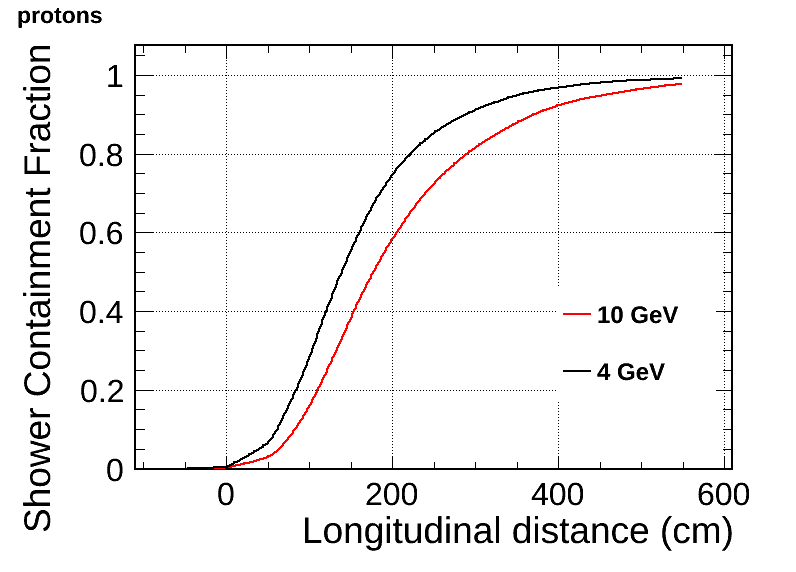
\includegraphics[width=0.49\textwidth,height=4.9cm]{protons_lcont_overlay}&
   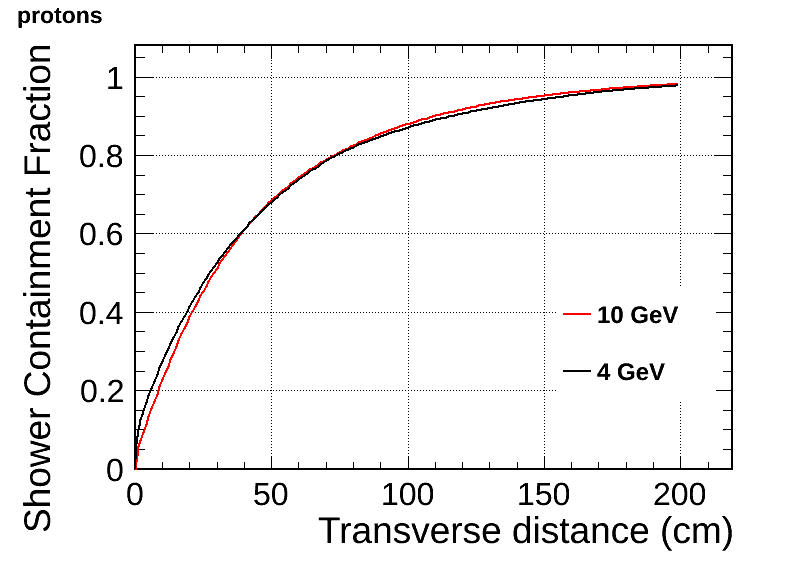
\includegraphics[width=0.49\textwidth,height=4.9cm]{protons_wcont_overlay}\\
  \end{tabular}
\end{cdrfigure}


\item $e/\gamma$ separation for reconstruction algorithms already incorporated into ProtoDUNE.
\item Reconstruction efficiency for primary and secondary particles (from beam and cosmics).
\item $dQ/dx$ and $dQ/dx$ vs. range for charge particles (protons, pion, muon, kaon)

Information on range and charge deposition for stopping charged-particles can be used to 
accurately identify particle type as well as measure kinetic energy. 
Fig.~\ref{fig:resrange}  (left) shows track energy loss per unit length \footnote{Signal attenuation due to recombination effect is not corrected for the PID purpose since it is a deterministic transformation which does not add measurement information.}
($dQ/dx$) as a function of residual 
track range for simulated muon, pion, proton and kaon particle tracks. 
A neural-net-based algorithm~\cite{nn_pid,rd_pid}
was used to determine PID functions for each particle hypothesis.

Fig.~\ref{fig:resrange} (right) 
shows the distribution of reconstructed $dQ/dx$ in a narrow bin of residual range 6($\pm$1)cm to illustrate the scale of difference between particle types. Proton and kaon bands are well separated from each other and from pion and muon bands, while pion and muon bands are almost overlapping which is challenging for the efficient separation. 
Simulation is performed with
FLUKA~\cite{fluka05} and ICARUS geometry (3-mm wire pitch) and reconstruction code~\cite{icarus_reco}.


The PID efficiency and purity will  depend on the detector configuration, geometry and 
reconstruction algorithm. The DUNE APA configuration and reconstruction algorithms
may give significantly different results, especially for pion/muon separation. 
It is therefore important to test PID in a realistic prototype detector
data in the presence of all detector effects.
Event samples that include an adequate number of stopping particles for each species
(muon, pions, protons and kaons) are included in the particle summary request in order to 
perform tests of PID algorithms and Bethe-Bloch calibration measurements.

\begin{cdrfigure}[ICARUS simulated track $dQ/dx$]{resrange}{ICARUS simulated track $dQ/dx$ as a function of residual range for muons, pions, protons and kaons, used as training data in a neutral-net-based PID algorithm (left). Distribution of $dQ/dx$ for each particle type for a bin with residual range 
6($\pm$1)~cm (right). The small difference between muon and pion PID is illustrated.}
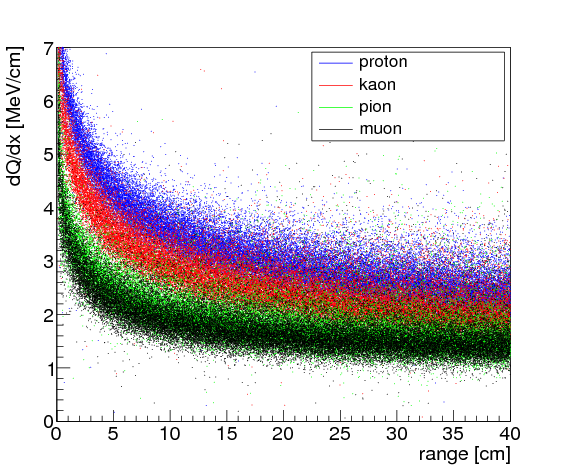
\includegraphics[width=0.53\textwidth,height=6.0cm]{pids_new}
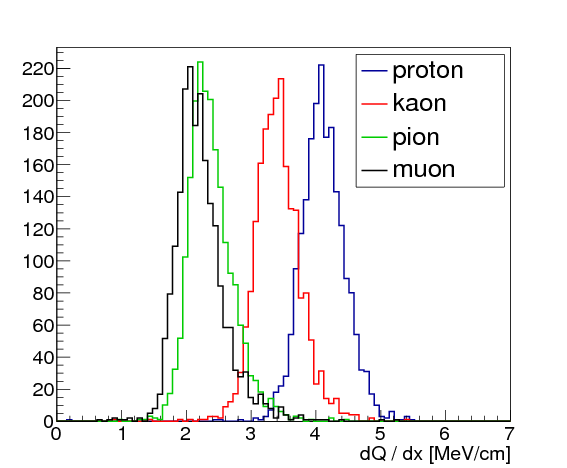
\includegraphics[width=0.46\textwidth,height=6.0cm]{prkpimu_new}
\end{cdrfigure}


\item Fraction of true energy deposited by interacting charge particles 
The measured energy deposition for various particles and its dependence on the direction of the particle will be used to tune
MC simulations and allow improvements to reconstruction of neutrino energy and interaction topologies. % with good particle identification.
Measurements of the response to charged particles and
photons with the DUNE-PT will extend and be complementary to
measurements made with other smaller detectors, such as LArIAT \cite{LArIAT}
and CAPTAIN~\cite{captain}.
\fixme{what's the DUNE-PT?}

\item Differences in mean energy deposited and width of visible energy  for interacting particles.
\item $\Delta X, \Delta Y$ and $\Delta Z$ due to  field distortion effects. 
\end{itemize}

%%%%%%%%%%%%%%%%%%%%%%%%%%%%%%%%%%%%%%%%%%%%%%
\section{Evaluation of event reconstruction performance}


%In the following, we define the goals that we aim to achieve regarding the TPC electronic noise and signal processing.
This section describes the goals defined for the TPC electronic noise and signal processing.
\fixme{goals or requirements? }
\begin{itemize}
\item The number of unusable channels is required to be smaller than 1\%: \\
All the past large LArTPC experiments (ICARUS, MicroBooNE, and DUNE-35ton) have suffered from a sizable
number of unusable channels ($>$ 10\%) for %due to various 
reasons such as high noise, dead electronics, 
and disconnected wires. At the same time, successes have been achieved for various subsystems in 
different experiments. \fixme{successes related to dead channels?}
For example, ICARUS has no disconnected wires. In LAriat, all 
cold electronics channels ($\sim$ 500) are live and achieve the expected $\sim$400 electrons equivalent 
noise charge (ENC). In the ATLAS LAr calorimeter, only about 0.1\% of the cold electronics channels are unusable. 
In MicroBooNE, the ENC after software noise filtering is about 400 electrons, which is consistent with 
the design specification of the cold electronics. In addition, all the major sources of electronic noise
have been identified and hardware solutions are in order. Therefore, with careful and systematic 
quality assurance and controls, it is definitely possible to reduce the total number of unusable channels
by at least one oder of magnitude. This is one of the primary goal of ProtoDUNE.

\fixme{the above is not clear. 

It needs a progression something like this:
`All these detectors have had channel problems. Problems have been identified and are fixed. From this we know we can reduce unusable channels by order of magnitude.' The sentence about successes is confusing: success after fixing? Or success in other areas?
}

\item The ENC generated beyond the cold preamplifier is required to negligible ($<$ 50\%~\footnote{Since the 
noises are added in quadrature, an extra electronic noise with less than 50\% of intrinsic cold preamplier
noise would lead to less than 10\% increase of the total noise.}) compared to the 
expected ENC generated from the cold preamplifier in $>$ 95\% of the channels: \\
The only irreducible electronics noise is coming from the preamplifier on the TPC wires. It is thus
crucial to optimize the overall system to reduce the noises generating from other sub-systems. 
LAriat acehived such a performance with about a total of 500 channels. 
\fixme{the `noises' is awkward. Can you say `the noise from each source is added in quadrature, an extra noise source with less than...?}
\item A robust procedure to validate the TPC field response function is required
be developed: \\
Field response on the induction plane is very complicated, but holds the key to achieve a robust TPC 
signal processing and thus the overall event reconstruction. It is therefore important to develop a 
program to calculate, calibrate, and validate field response functions. This validation of the field response function 
can be achieved by comparing the measured average response functions for cosmic muons with the simulated
ones. 
\item The overall signal calibration process is required to be validated: \\
The goal of the signal calibration process is to recover the number of ionized electrons based on
the digitized TPC waveform; this is the first step in the overall event reconstruction. It is crucial to 
validate that such a procedure is robust. This validation can be achieved by comparing the 
images from the raw digits with the images after the deconvolution procedure.
\end{itemize}




%%%%%%%%%%%%%%%%%%%%%%%%%%%%%%%%%%%%%%%%%%%%%%
\section{Particle interactions and cross sections}



Final state pions are produced copiously in neutrino interactions in the energy range for the DUNE beam  and contribute 
substantially to the total visible energy in the interaction.
These particles can re-interact either in the nuclear medium or after emerging from the target nucleus
and substantially change the visible energy deposited in the event. 
The importance of modeling final-state pion interactions on reconstructed neutrino energy has 
been recently demonstrated in the NuMI and Booster beam energy ranges~\cite{miniboonefsi, minervafsi}. \fixme{The `importance' or the modeling has been demonstrated? }

Detailed knowledge of pion-nucleus cross sections in the sub-GeV energy range is required in order
to tune generators~\cite{genie} to accurately model event visible energy. 
Existing data used to tune the models cover limited energies ($<$200~MeV) and are primarily on lighter target nuclei~\cite{fsirev}.
% need to check this reference from R. Ransom talk.
The requested $\pi^+$ and $\pi^-$ samples will allow new data samples for measuring
exclusive final state processes over the full relevant energy range and specifically on argon nuclei. \fixme{previous sentence unclear; is it about the `required' $\pi^+$ and $\pi^-$ samples?}
A high-statistics sample of charged particles will allow precise measurements of their interaction cross sections.

\begin{itemize}
\item pion interaction kinematics and cross sections
\item kaon interaction cross section to remove proton decay backgrounds


The DUNE experiment in the deep underground location will seek to detect several modes of proton decay.
%In particular, a first ever LAr detector 
This first-ever LAr detector of this scale underground will primarily improve sensitivity to 
proton decays with final state kaons such as  ${p \rightarrow K^+ \overline{\nu}}$. 
Sensitivity to this process is studied in~\cite{bueno}. $K^+$ detection efficiency is estimated to be $>$97\% in the
appropriate momentum range (500-800 MeV/c). The kaon samples requested in Table~\ref{tab:runsum} are needed in order to directly measure 
$K^+$ PID and detection efficiency. 

Obtaining low-energy kaons will likely be difficult in this beamline.
A sample of 13k beam kaons with 1~GeV/c momentum are requested \fixme{required?}  in order to provide 2k stopping $K^+$ track samples for PID studies.
(Only 15\% of $K^+$ stop at 1~GeV/c.)
A sizable sample of protons ($\sim 10^6$)
are requested \fixme{required} to study the possible background contributions to  $p \rightarrow K^+ \overline{\nu}$.
This sample of  protons are needed to quantify the possibility that an interacting proton 
is  misidentified as stopping kaon. A proton interaction which produces neutrals and one charged pion 
(which is misidentified or subsequently decays to $\mu$) can fake the final state kaon signal.

\fixme{attempted rewrite of above pgraph:}
In order to provide the needed 2000 stopping $K^+$ track samples for the PID studies, a sample of 13k beam kaons with 1~GeV/c momentum must be obtained, which will likely be difficult in this beamline. (Only 15\% of $K^+$ stop at 1~GeV/c.)
A sizable sample of protons ($\sim 10^6$)
is also needed. This will allow study of the possible background contributions to $p \rightarrow K^+ \overline{\nu}$ in order to quantify the probability of an interacting proton 
being misidentified as stopping kaon. A proton interaction that produces neutrals and one charged pion 
(that is misidentified or subsequently decays to $\mu$) can fake the final-state kaon signal.

\item muon capture for charge identification

It is not possible to determine the charge of the particle on an event-by-event basis with non-magnetized LArTPC detectors. A statistical separation will be studied which will make use of differences in muon versus anti-muon capture cross sections and lifetime.
%However, the statistical analyst will be possible. We will fit the muon's half time which is different for muons and antimony due to different muon capture cross sections. 
For the $\mu^-$ we expect about 99.9\% to be captured on argon whereas essentially all $\mu^+$ decay \cite{stopmu}.
Charge-sign tagged $\nu_\mu$ samples may be useful to constrain exotic possibilities such as
non-standard neutrino interactions which predict differences in the particle and anti-particle survival probabilities. 

\fixme{attempted rewrite of above pgraph:}
With non-magnetized LArTPC detectors it is not possible to determine particle charge on an event-by-event basis. Therefore, a statistical separation that makes use of differences in muon versus antimuon capture cross sections and lifetime will be investigated.
About 99.9\% of $\mu^-$'s are expected to be captured on argon, compared to essentially all $\mu^+$ decays~\cite{stopmu}.
Charge-sign tagged $\nu_\mu$ samples, which predict differences in the particle and antiparticle survival probabilities, may be useful for constraining exotic possibilities, such as non-standard neutrino interactions. 


\item Supernova and Michel electrons

Neutrinos produced in supernova burst (SNB) explosions are calculated to be in the few-to-30-MeV range.
The DUNE Far Detector is expected to have unique sensitivity to the $\nu_e$'s from a SNB in our galaxy.
%
The test beam cannot offer a sample of  such low-energy electrons, but Michel electrons  produced by 
decaying stopped muons are ideal for calibrating electron response in the appropriate 10-50~MeV energy range. 
The requested \fixme{required}  sample of low-energy muons will supply the 1400 Michel electrons required for a 1\% 
calibration of electrons in this energy range. This sample can be compared to a similar Michel electron sample
stemming from stopping cosmic muons.

\end{itemize}



%%%%%%%%%%%%%%%%%%%%%%%%%%%%%%%%%%%%%%%%%%%%%%
\section{Detector engineering validation}
engineering motivation

%%%%%%%%%%%%%%%%%%%%%%%%%%%%%%%%%%%%%%%%%%%%%%
\section{Installation validation}




